% Options for packages loaded elsewhere
\PassOptionsToPackage{unicode}{hyperref}
\PassOptionsToPackage{hyphens}{url}
\PassOptionsToPackage{dvipsnames,svgnames,x11names}{xcolor}
%
\documentclass[
  letterpaper,
  DIV=11,
  numbers=noendperiod]{scrartcl}

\usepackage{amsmath,amssymb}
\usepackage{lmodern}
\usepackage{iftex}
\ifPDFTeX
  \usepackage[T1]{fontenc}
  \usepackage[utf8]{inputenc}
  \usepackage{textcomp} % provide euro and other symbols
\else % if luatex or xetex
  \usepackage{unicode-math}
  \defaultfontfeatures{Scale=MatchLowercase}
  \defaultfontfeatures[\rmfamily]{Ligatures=TeX,Scale=1}
\fi
% Use upquote if available, for straight quotes in verbatim environments
\IfFileExists{upquote.sty}{\usepackage{upquote}}{}
\IfFileExists{microtype.sty}{% use microtype if available
  \usepackage[]{microtype}
  \UseMicrotypeSet[protrusion]{basicmath} % disable protrusion for tt fonts
}{}
\makeatletter
\@ifundefined{KOMAClassName}{% if non-KOMA class
  \IfFileExists{parskip.sty}{%
    \usepackage{parskip}
  }{% else
    \setlength{\parindent}{0pt}
    \setlength{\parskip}{6pt plus 2pt minus 1pt}}
}{% if KOMA class
  \KOMAoptions{parskip=half}}
\makeatother
\usepackage{xcolor}
\setlength{\emergencystretch}{3em} % prevent overfull lines
\setcounter{secnumdepth}{-\maxdimen} % remove section numbering
% Make \paragraph and \subparagraph free-standing
\ifx\paragraph\undefined\else
  \let\oldparagraph\paragraph
  \renewcommand{\paragraph}[1]{\oldparagraph{#1}\mbox{}}
\fi
\ifx\subparagraph\undefined\else
  \let\oldsubparagraph\subparagraph
  \renewcommand{\subparagraph}[1]{\oldsubparagraph{#1}\mbox{}}
\fi

\usepackage{color}
\usepackage{fancyvrb}
\newcommand{\VerbBar}{|}
\newcommand{\VERB}{\Verb[commandchars=\\\{\}]}
\DefineVerbatimEnvironment{Highlighting}{Verbatim}{commandchars=\\\{\}}
% Add ',fontsize=\small' for more characters per line
\usepackage{framed}
\definecolor{shadecolor}{RGB}{241,243,245}
\newenvironment{Shaded}{\begin{snugshade}}{\end{snugshade}}
\newcommand{\AlertTok}[1]{\textcolor[rgb]{0.68,0.00,0.00}{#1}}
\newcommand{\AnnotationTok}[1]{\textcolor[rgb]{0.37,0.37,0.37}{#1}}
\newcommand{\AttributeTok}[1]{\textcolor[rgb]{0.40,0.45,0.13}{#1}}
\newcommand{\BaseNTok}[1]{\textcolor[rgb]{0.68,0.00,0.00}{#1}}
\newcommand{\BuiltInTok}[1]{\textcolor[rgb]{0.00,0.23,0.31}{#1}}
\newcommand{\CharTok}[1]{\textcolor[rgb]{0.13,0.47,0.30}{#1}}
\newcommand{\CommentTok}[1]{\textcolor[rgb]{0.37,0.37,0.37}{#1}}
\newcommand{\CommentVarTok}[1]{\textcolor[rgb]{0.37,0.37,0.37}{\textit{#1}}}
\newcommand{\ConstantTok}[1]{\textcolor[rgb]{0.56,0.35,0.01}{#1}}
\newcommand{\ControlFlowTok}[1]{\textcolor[rgb]{0.00,0.23,0.31}{#1}}
\newcommand{\DataTypeTok}[1]{\textcolor[rgb]{0.68,0.00,0.00}{#1}}
\newcommand{\DecValTok}[1]{\textcolor[rgb]{0.68,0.00,0.00}{#1}}
\newcommand{\DocumentationTok}[1]{\textcolor[rgb]{0.37,0.37,0.37}{\textit{#1}}}
\newcommand{\ErrorTok}[1]{\textcolor[rgb]{0.68,0.00,0.00}{#1}}
\newcommand{\ExtensionTok}[1]{\textcolor[rgb]{0.00,0.23,0.31}{#1}}
\newcommand{\FloatTok}[1]{\textcolor[rgb]{0.68,0.00,0.00}{#1}}
\newcommand{\FunctionTok}[1]{\textcolor[rgb]{0.28,0.35,0.67}{#1}}
\newcommand{\ImportTok}[1]{\textcolor[rgb]{0.00,0.46,0.62}{#1}}
\newcommand{\InformationTok}[1]{\textcolor[rgb]{0.37,0.37,0.37}{#1}}
\newcommand{\KeywordTok}[1]{\textcolor[rgb]{0.00,0.23,0.31}{#1}}
\newcommand{\NormalTok}[1]{\textcolor[rgb]{0.00,0.23,0.31}{#1}}
\newcommand{\OperatorTok}[1]{\textcolor[rgb]{0.37,0.37,0.37}{#1}}
\newcommand{\OtherTok}[1]{\textcolor[rgb]{0.00,0.23,0.31}{#1}}
\newcommand{\PreprocessorTok}[1]{\textcolor[rgb]{0.68,0.00,0.00}{#1}}
\newcommand{\RegionMarkerTok}[1]{\textcolor[rgb]{0.00,0.23,0.31}{#1}}
\newcommand{\SpecialCharTok}[1]{\textcolor[rgb]{0.37,0.37,0.37}{#1}}
\newcommand{\SpecialStringTok}[1]{\textcolor[rgb]{0.13,0.47,0.30}{#1}}
\newcommand{\StringTok}[1]{\textcolor[rgb]{0.13,0.47,0.30}{#1}}
\newcommand{\VariableTok}[1]{\textcolor[rgb]{0.07,0.07,0.07}{#1}}
\newcommand{\VerbatimStringTok}[1]{\textcolor[rgb]{0.13,0.47,0.30}{#1}}
\newcommand{\WarningTok}[1]{\textcolor[rgb]{0.37,0.37,0.37}{\textit{#1}}}

\providecommand{\tightlist}{%
  \setlength{\itemsep}{0pt}\setlength{\parskip}{0pt}}\usepackage{longtable,booktabs,array}
\usepackage{calc} % for calculating minipage widths
% Correct order of tables after \paragraph or \subparagraph
\usepackage{etoolbox}
\makeatletter
\patchcmd\longtable{\par}{\if@noskipsec\mbox{}\fi\par}{}{}
\makeatother
% Allow footnotes in longtable head/foot
\IfFileExists{footnotehyper.sty}{\usepackage{footnotehyper}}{\usepackage{footnote}}
\makesavenoteenv{longtable}
\usepackage{graphicx}
\makeatletter
\def\maxwidth{\ifdim\Gin@nat@width>\linewidth\linewidth\else\Gin@nat@width\fi}
\def\maxheight{\ifdim\Gin@nat@height>\textheight\textheight\else\Gin@nat@height\fi}
\makeatother
% Scale images if necessary, so that they will not overflow the page
% margins by default, and it is still possible to overwrite the defaults
% using explicit options in \includegraphics[width, height, ...]{}
\setkeys{Gin}{width=\maxwidth,height=\maxheight,keepaspectratio}
% Set default figure placement to htbp
\makeatletter
\def\fps@figure{htbp}
\makeatother

\KOMAoption{captions}{tableheading}
\makeatletter
\makeatother
\makeatletter
\makeatother
\makeatletter
\@ifpackageloaded{caption}{}{\usepackage{caption}}
\AtBeginDocument{%
\ifdefined\contentsname
  \renewcommand*\contentsname{Table of contents}
\else
  \newcommand\contentsname{Table of contents}
\fi
\ifdefined\listfigurename
  \renewcommand*\listfigurename{List of Figures}
\else
  \newcommand\listfigurename{List of Figures}
\fi
\ifdefined\listtablename
  \renewcommand*\listtablename{List of Tables}
\else
  \newcommand\listtablename{List of Tables}
\fi
\ifdefined\figurename
  \renewcommand*\figurename{Figure}
\else
  \newcommand\figurename{Figure}
\fi
\ifdefined\tablename
  \renewcommand*\tablename{Table}
\else
  \newcommand\tablename{Table}
\fi
}
\@ifpackageloaded{float}{}{\usepackage{float}}
\floatstyle{ruled}
\@ifundefined{c@chapter}{\newfloat{codelisting}{h}{lop}}{\newfloat{codelisting}{h}{lop}[chapter]}
\floatname{codelisting}{Listing}
\newcommand*\listoflistings{\listof{codelisting}{List of Listings}}
\makeatother
\makeatletter
\@ifpackageloaded{caption}{}{\usepackage{caption}}
\@ifpackageloaded{subcaption}{}{\usepackage{subcaption}}
\makeatother
\makeatletter
\@ifpackageloaded{tcolorbox}{}{\usepackage[many]{tcolorbox}}
\makeatother
\makeatletter
\@ifundefined{shadecolor}{\definecolor{shadecolor}{rgb}{.97, .97, .97}}
\makeatother
\makeatletter
\makeatother
\ifLuaTeX
  \usepackage{selnolig}  % disable illegal ligatures
\fi
\IfFileExists{bookmark.sty}{\usepackage{bookmark}}{\usepackage{hyperref}}
\IfFileExists{xurl.sty}{\usepackage{xurl}}{} % add URL line breaks if available
\urlstyle{same} % disable monospaced font for URLs
\hypersetup{
  pdftitle={AdvancedStatsAssignment},
  colorlinks=true,
  linkcolor={blue},
  filecolor={Maroon},
  citecolor={Blue},
  urlcolor={Blue},
  pdfcreator={LaTeX via pandoc}}

\title{AdvancedStatsAssignment}
\author{}
\date{}

\begin{document}
\maketitle
\ifdefined\Shaded\renewenvironment{Shaded}{\begin{tcolorbox}[sharp corners, interior hidden, enhanced, frame hidden, borderline west={3pt}{0pt}{shadecolor}, boxrule=0pt, breakable]}{\end{tcolorbox}}\fi

\hypertarget{question-1}{%
\subsection{Question 1}\label{question-1}}

\begin{Shaded}
\begin{Highlighting}[]
\FunctionTok{source}\NormalTok{(}\StringTok{"ScotlandMap.R"}\NormalTok{)  }\CommentTok{\# need to read in the Scotland Map function}
\NormalTok{testdat }\OtherTok{\textless{}{-}} \FunctionTok{runif}\NormalTok{(}\DecValTok{56}\NormalTok{)  }\CommentTok{\# generate random numbers to use as observations}
\FunctionTok{ScotlandMap}\NormalTok{(testdat, }\AttributeTok{figtitle =} \StringTok{"Scotland random numbers"}\NormalTok{)}
\end{Highlighting}
\end{Shaded}

\hypertarget{question-1-a}{%
\subsection{Question 1 a)}\label{question-1-a}}

\begin{Shaded}
\begin{Highlighting}[]
\NormalTok{ScotlandDF}\SpecialCharTok{$}\NormalTok{SMR }\OtherTok{=}\NormalTok{ ScotlandDF}\SpecialCharTok{$}\NormalTok{Observed}\SpecialCharTok{/}\NormalTok{ScotlandDF}\SpecialCharTok{$}\NormalTok{Expected}
\end{Highlighting}
\end{Shaded}

\begin{Shaded}
\begin{Highlighting}[]
\FunctionTok{hist}\NormalTok{(ScotlandDF}\SpecialCharTok{$}\NormalTok{SMR, }\AttributeTok{breaks =} \DecValTok{20}\NormalTok{, }\AttributeTok{col =} \StringTok{"lightblue"}\NormalTok{, }\AttributeTok{main =} \StringTok{"Distribution of Standard Mortality Ratios"}\NormalTok{,}
    \AttributeTok{xlab =} \StringTok{"SMR"}\NormalTok{)}
\end{Highlighting}
\end{Shaded}

\begin{figure}[H]

{\centering 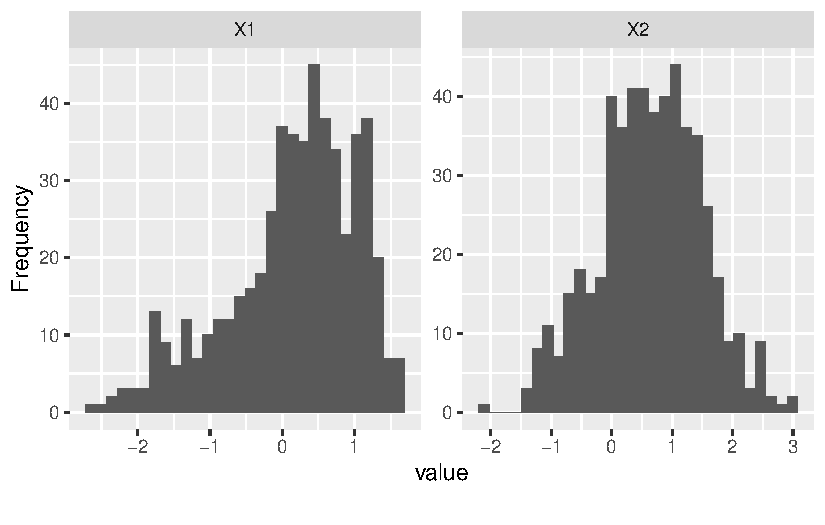
\includegraphics{AssignmentAdvancedTopicsInStatistics_files/figure-pdf/unnamed-chunk-4-1.pdf}

}

\end{figure}

\begin{Shaded}
\begin{Highlighting}[]
\FunctionTok{source}\NormalTok{(}\StringTok{"ScotlandMap.R"}\NormalTok{)  }\CommentTok{\# need to read in the ScotlandMap function}
\NormalTok{testdat }\OtherTok{\textless{}{-}}\NormalTok{ ScotlandDF}\SpecialCharTok{$}\NormalTok{SMR  }\CommentTok{\# generate random numbers to use as observations}
\FunctionTok{ScotlandMap}\NormalTok{(testdat, }\AttributeTok{figtitle =} \StringTok{"Scotland random numbers"}\NormalTok{)}
\end{Highlighting}
\end{Shaded}

\begin{verbatim}
Warning: OGR support is provided by the sf and terra packages among others
\end{verbatim}

\begin{verbatim}
Warning: OGR support is provided by the sf and terra packages among others
\end{verbatim}

\begin{verbatim}
Warning: OGR support is provided by the sf and terra packages among others
\end{verbatim}

\begin{verbatim}
Warning: OGR support is provided by the sf and terra packages among others
\end{verbatim}

\begin{verbatim}
Warning: OGR support is provided by the sf and terra packages among others
\end{verbatim}

\begin{verbatim}
Warning: OGR support is provided by the sf and terra packages among others
\end{verbatim}

\begin{verbatim}
OGR data source with driver: ESRI Shapefile 
Source: "C:\AppliedDataScienceAndStatistics\Applied-Data-Science-and-Statistics\Term2\AdvancedTopicsInStatistics\Assignment", layer: "Scotland"
with 56 features
It has 1 fields
\end{verbatim}

\begin{figure}[H]

{\centering 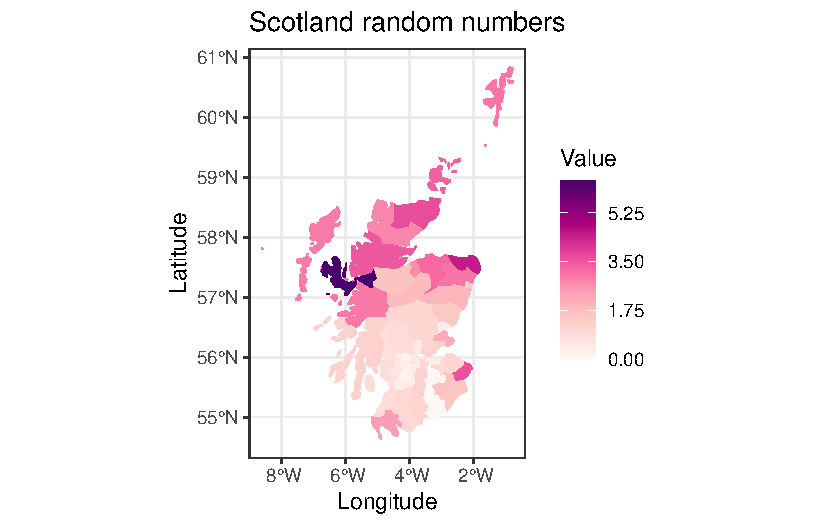
\includegraphics{AssignmentAdvancedTopicsInStatistics_files/figure-pdf/unnamed-chunk-5-1.pdf}

}

\end{figure}

\hypertarget{question-1-b}{%
\subsection{Question 1 b)}\label{question-1-b}}

For the model: \begin{align*}
Obs_i \sim \text{Pois}(\mu_i) \
\log(\mu_i) = \log(\text{Exp}_i) + \beta_0 + \theta_i \
\text{RR}_i = \exp(\beta_0) \exp(\theta_i)
\end{align*}= \log(\text{Exp}\_i) + \beta\_0 + \theta\_i\\
\text{RR}\_i = \exp(\beta\_0) \exp(\theta\_i)
\textbackslash end\{align*\}

\(\beta0\) is the intercept that represents the baseline for when all
the other variables are 0 which can also be interpreted as the log
number expected of cases per administrative area.

\(\theta i\) is the effect that captures the variation in the observed
number of cases that cannot be explained by the expected numbers alone.
\(\theta i\) also represents the deviation of the log observed number of
cases from the log expected number of cases for area i.

In the Poisson model, \(\theta i\) represents the deviation of the
observed number of cases in area i from the expected number of cases in
area i, given the reference rates. In other words, it captures how much
higher or lower the observed number of cases is compared to what we
would expect based on the reference rates

The role of θi in the estimation of the relative risk is to allow for
variation in the risk of disease across different areas, over and above
what is explained by the reference rates. By including a random effect
for each area in the model, we are able to estimate the relative risk
for each area, while accounting for the fact that some areas may have
higher or lower risk due to factors that are not captured by the
reference rates alone.

\hypertarget{question-2---classification}{%
\subsection{Question 2 -
classification}\label{question-2---classification}}

\hypertarget{question-2.1}{%
\subsection{Question 2.1}\label{question-2.1}}

Group 0 is characterised for always having x1 \textgreater{} -1,65 and
x2 \textless{} 2,05 with the majority of the occurences of group 0
having

\begin{Shaded}
\begin{Highlighting}[]
\DocumentationTok{\#\# I am just going to split the dataframe in two so its easier to show}
\DocumentationTok{\#\# an histogram of each variable for both groups}

\NormalTok{group0 }\OtherTok{\textless{}{-}} \FunctionTok{subset}\NormalTok{(classificationDF, Group }\SpecialCharTok{==} \DecValTok{0}\NormalTok{)}
\NormalTok{group1 }\OtherTok{\textless{}{-}} \FunctionTok{subset}\NormalTok{(classificationDF, Group }\SpecialCharTok{==} \DecValTok{1}\NormalTok{)}

\DocumentationTok{\#\# removing the id variable from both of these new data frames so they}
\DocumentationTok{\#\# are not included in the histograms}
\NormalTok{group0 }\OtherTok{=}\NormalTok{ group0 }\SpecialCharTok{\%\textgreater{}\%}
    \FunctionTok{select}\NormalTok{(}\SpecialCharTok{{-}}\NormalTok{(}\DecValTok{1}\NormalTok{))}
\NormalTok{group1 }\OtherTok{=}\NormalTok{ group1 }\SpecialCharTok{\%\textgreater{}\%}
    \FunctionTok{select}\NormalTok{(}\SpecialCharTok{{-}}\NormalTok{(}\DecValTok{1}\NormalTok{))}


\FunctionTok{plot\_histogram}\NormalTok{(group0)}
\end{Highlighting}
\end{Shaded}

\begin{figure}[H]

{\centering 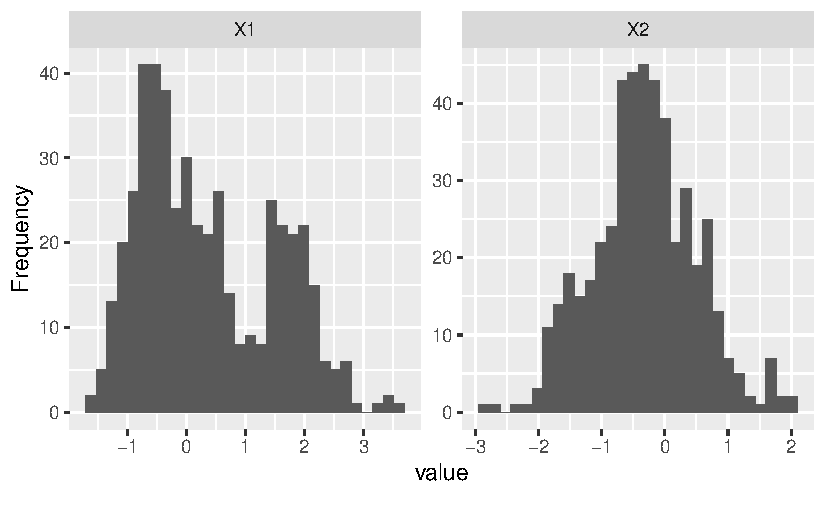
\includegraphics{AssignmentAdvancedTopicsInStatistics_files/figure-pdf/unnamed-chunk-16-1.pdf}

}

\end{figure}

As we can see from the histograms from group 0 it seems that X2 seems to
follow a normal distribution that is very slightly skewed to the left
and has mean -0,5. X1 is clearly skewed to the right possibly following
a normal distribution and again mean equal to -0,5.

\begin{Shaded}
\begin{Highlighting}[]
\FunctionTok{plot\_histogram}\NormalTok{(group1)}
\end{Highlighting}
\end{Shaded}

\begin{figure}[H]

{\centering 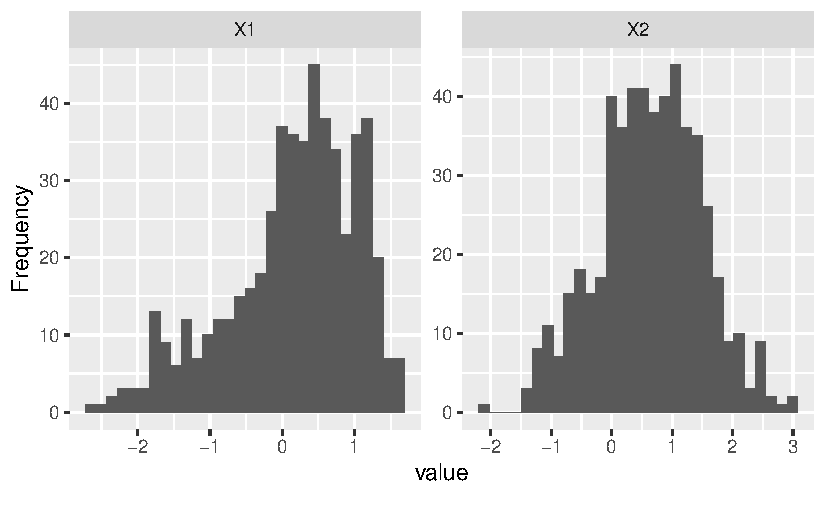
\includegraphics{AssignmentAdvancedTopicsInStatistics_files/figure-pdf/unnamed-chunk-17-1.pdf}

}

\end{figure}

Group 1 histograms reveal that X2 is normally distributed with mean
equal to 0,5 and sightly skewed to the left. The variable X1 also seems
to follow a normal distribution that has a very prolonged skewness to
the left and mean 0,5.0

\hypertarget{question-2.2}{%
\subsection{Question 2.2}\label{question-2.2}}

Both LDA and QDA assume normality which is true from what we can see
from the histograms on 2.1

Starting with Linear discriminant analysis (LDA) we can easily see from
the initial graph that we can see that the any sensible decision
boundary is highly non-linear. As analysed from histograms this data
violates the initial assumption of homogeneity of variance
(homoscedasticity). The non-linearity of the data would also lead to LDA
having terrible performance. As such we can conclude that LDA is not
suitable for this data.

Secondly, quadratic discriminant analysis (QDA) follow the assumption of
normality of each of the variables which does seem to hold even with how
highly non-linear the data is. However judging from the plot with the
observations, it does seem that QDA might not have enough flexibility to
account for all the variability in what is the theoretical Bayes
decision boundary. As such QDA could be appropriate for this data but
not the best performing classification method for such data.

Thirdly, K-nearest neighbour classification (KNN) has no assumptions
made about the shape of the decision, as such as we choose a adequate
level of smoothness to prevent overfitting KNN classification is an
adequate method for the data.

Support Vector Machines (SVM) are most commonly used for binary
classification, which holds true for our data. The high non-linear
decision boundary however requires a careful selection of a non linear
kernel function to ensure that the boundary becomes non-linear when
converted back to the regular space. As such I deem SVM an appropriate
method to classify the data.

Finally, Random forest works by constructing multiple decision trees
randomly selecting a portion of the variables and de-correlate them
using multiple bootstrapped sets. Since our data has only 2 variables
there isn't enough variables to overcome overfitting. To conclude,
Random Forest classification is not very appropriate to this type of
data.

\hypertarget{question-2.3}{%
\subsection{Question 2.3}\label{question-2.3}}

\begin{Shaded}
\begin{Highlighting}[]
\CommentTok{\# make this example reproducible}
\FunctionTok{set.seed}\NormalTok{(}\DecValTok{26041999}\NormalTok{)}
\CommentTok{\# use 80\% of dataset as training set and 20\% as test set}
\NormalTok{sample }\OtherTok{\textless{}{-}} \FunctionTok{sample.split}\NormalTok{(classificationDF}\SpecialCharTok{$}\NormalTok{Group, }\AttributeTok{SplitRatio =} \FloatTok{0.8}\NormalTok{)}
\DocumentationTok{\#\# note that the column selected above can be any column.}
\NormalTok{train }\OtherTok{\textless{}{-}}\NormalTok{ classificationDF[sample, ]}
\NormalTok{test }\OtherTok{\textless{}{-}}\NormalTok{ classificationDF[}\SpecialCharTok{!}\NormalTok{sample, ]}

\CommentTok{\# split the data using the indices returned by the createDataPartition}
\CommentTok{\# function}
\NormalTok{X\_train }\OtherTok{\textless{}{-}}\NormalTok{ train[, }\FunctionTok{c}\NormalTok{(}\StringTok{"X1"}\NormalTok{, }\StringTok{"X2"}\NormalTok{)]}
\NormalTok{y\_train }\OtherTok{\textless{}{-}}\NormalTok{ train}\SpecialCharTok{$}\NormalTok{Group}
\NormalTok{X\_test }\OtherTok{\textless{}{-}}\NormalTok{ test[, }\FunctionTok{c}\NormalTok{(}\StringTok{"X1"}\NormalTok{, }\StringTok{"X2"}\NormalTok{)]}
\NormalTok{y\_test }\OtherTok{\textless{}{-}}\NormalTok{ test}\SpecialCharTok{$}\NormalTok{Group}

\CommentTok{\# check the dimensions}
\FunctionTok{dim}\NormalTok{(train)}
\end{Highlighting}
\end{Shaded}

\begin{verbatim}
[1] 800   4
\end{verbatim}

\begin{Shaded}
\begin{Highlighting}[]
\FunctionTok{dim}\NormalTok{(test)}
\end{Highlighting}
\end{Shaded}

\begin{verbatim}
[1] 200   4
\end{verbatim}

\hypertarget{question-2.4}{%
\subsection{Question 2.4}\label{question-2.4}}

The 3 method I will be using are QDA, KNN and SVM as deemed to be the
most appropriate methods for this data.

\hypertarget{qda---quadratic-discriminant-analysis}{%
\subsection{QDA - quadratic discriminant
analysis}\label{qda---quadratic-discriminant-analysis}}

\hypertarget{knn---k-nearest-neighbour}{%
\subsection{KNN - K-nearest neighbour}\label{knn---k-nearest-neighbour}}

\begin{Shaded}
\begin{Highlighting}[]
\CommentTok{\# fit the model}
\NormalTok{fit }\OtherTok{=} \FunctionTok{knn}\NormalTok{(}\AttributeTok{train =}\NormalTok{ X\_train, }\AttributeTok{test =}\NormalTok{ X\_test, }\AttributeTok{cl =}\NormalTok{ y\_train, }\AttributeTok{k =} \DecValTok{3}\NormalTok{)}
\CommentTok{\# fit = knn(xTrain,xTest,yTrain,k=3)}

\CommentTok{\# produce the confusion matrix when numbers are used as class labels we}
\CommentTok{\# might need}
\NormalTok{confusion }\OtherTok{=} \FunctionTok{confusionMatrix}\NormalTok{(}\FunctionTok{as.factor}\NormalTok{(fit), }\FunctionTok{as.factor}\NormalTok{(y\_test))}

\NormalTok{confusion}
\end{Highlighting}
\end{Shaded}

\begin{verbatim}
Confusion Matrix and Statistics

          Reference
Prediction  0  1
         0 80 17
         1 15 88
                                          
               Accuracy : 0.84            
                 95% CI : (0.7817, 0.8879)
    No Information Rate : 0.525           
    P-Value [Acc > NIR] : <2e-16          
                                          
                  Kappa : 0.6795          
                                          
 Mcnemar's Test P-Value : 0.8597          
                                          
            Sensitivity : 0.8421          
            Specificity : 0.8381          
         Pos Pred Value : 0.8247          
         Neg Pred Value : 0.8544          
             Prevalence : 0.4750          
         Detection Rate : 0.4000          
   Detection Prevalence : 0.4850          
      Balanced Accuracy : 0.8401          
                                          
       'Positive' Class : 0               
                                          
\end{verbatim}

\begin{Shaded}
\begin{Highlighting}[]
\NormalTok{test}\SpecialCharTok{$}\NormalTok{predicted\_group }\OtherTok{\textless{}{-}}\NormalTok{ fit}
\NormalTok{test}\SpecialCharTok{$}\NormalTok{correct\_prediction }\OtherTok{\textless{}{-}}\NormalTok{ test}\SpecialCharTok{$}\NormalTok{predicted\_group }\SpecialCharTok{==}\NormalTok{ test}\SpecialCharTok{$}\NormalTok{Group}

\CommentTok{\# plot the data points}
\NormalTok{p }\OtherTok{\textless{}{-}} \FunctionTok{ggplot}\NormalTok{() }\SpecialCharTok{+} \FunctionTok{geom\_point}\NormalTok{(}\AttributeTok{data =}\NormalTok{ train, }\FunctionTok{aes}\NormalTok{(}\AttributeTok{x =}\NormalTok{ X1, }\AttributeTok{y =}\NormalTok{ X2, }\AttributeTok{color =} \StringTok{"Training"}\NormalTok{),}
    \AttributeTok{size =} \DecValTok{3}\NormalTok{) }\SpecialCharTok{+} \FunctionTok{geom\_point}\NormalTok{(}\AttributeTok{data =}\NormalTok{ test, }\FunctionTok{aes}\NormalTok{(}\AttributeTok{x =}\NormalTok{ X1, }\AttributeTok{y =}\NormalTok{ X2, }\AttributeTok{color =}\NormalTok{ correct\_prediction,}
    \AttributeTok{shape =} \FunctionTok{factor}\NormalTok{(correct\_prediction)), }\AttributeTok{size =} \DecValTok{3}\NormalTok{) }\SpecialCharTok{+} \FunctionTok{scale\_color\_manual}\NormalTok{(}\AttributeTok{values =} \FunctionTok{c}\NormalTok{(}\StringTok{"red"}\NormalTok{,}
    \StringTok{"blue"}\NormalTok{, }\StringTok{"green"}\NormalTok{), }\AttributeTok{labels =} \FunctionTok{c}\NormalTok{(}\StringTok{"Incorrect"}\NormalTok{, }\StringTok{"Correct"}\NormalTok{, }\StringTok{"Training"}\NormalTok{)) }\SpecialCharTok{+} \FunctionTok{scale\_shape\_manual}\NormalTok{(}\AttributeTok{values =} \FunctionTok{c}\NormalTok{(}\DecValTok{1}\NormalTok{,}
    \DecValTok{16}\NormalTok{)) }\SpecialCharTok{+} \FunctionTok{labs}\NormalTok{(}\AttributeTok{x =} \StringTok{"X1"}\NormalTok{, }\AttributeTok{y =} \StringTok{"X2"}\NormalTok{, }\AttributeTok{color =} \StringTok{""}\NormalTok{, }\AttributeTok{shape =} \StringTok{""}\NormalTok{) }\SpecialCharTok{+} \FunctionTok{ggtitle}\NormalTok{(}\StringTok{"KNN Classification Results"}\NormalTok{)}

\CommentTok{\# display the plot}
\FunctionTok{print}\NormalTok{(p)}
\end{Highlighting}
\end{Shaded}

\begin{figure}[H]

{\centering 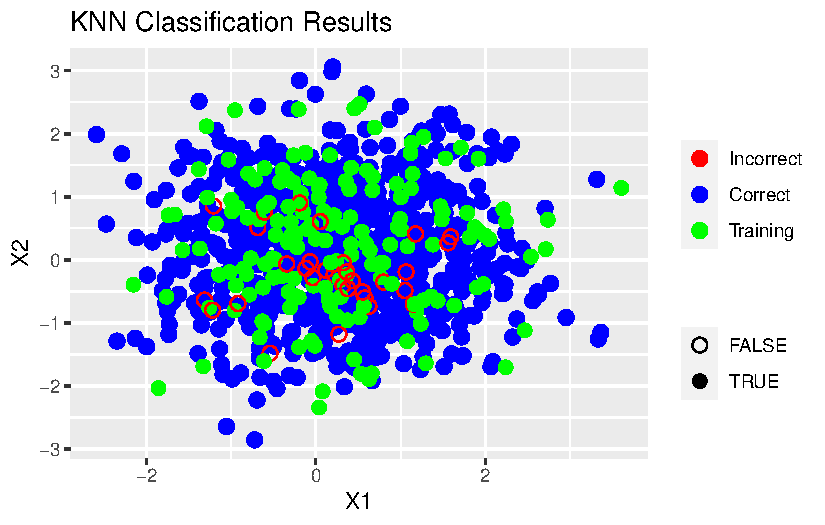
\includegraphics{AssignmentAdvancedTopicsInStatistics_files/figure-pdf/unnamed-chunk-21-1.pdf}

}

\end{figure}

\hypertarget{svm---support-vector-machines}{%
\subsection{SVM - Support Vector
Machines}\label{svm---support-vector-machines}}

\begin{Shaded}
\begin{Highlighting}[]
\DocumentationTok{\#\# checking the model performance with multiple difference C constants}
\NormalTok{mdl }\OtherTok{\textless{}{-}} \FunctionTok{train}\NormalTok{(}\AttributeTok{x =}\NormalTok{ X\_train, }\AttributeTok{y =}\NormalTok{ y\_train, }\AttributeTok{method =} \StringTok{"svmLinear"}\NormalTok{, }\AttributeTok{trControl =} \FunctionTok{trainControl}\NormalTok{(}\StringTok{"cv"}\NormalTok{,}
    \AttributeTok{number =} \DecValTok{5}\NormalTok{), }\AttributeTok{tuneGrid =} \FunctionTok{expand.grid}\NormalTok{(}\AttributeTok{C =} \FunctionTok{seq}\NormalTok{(}\DecValTok{0}\NormalTok{, }\DecValTok{2}\NormalTok{, }\AttributeTok{length =} \DecValTok{20}\NormalTok{)))}
\end{Highlighting}
\end{Shaded}

\begin{verbatim}
Warning in train.default(x = X_train, y = y_train, method = "svmLinear", : You
are trying to do regression and your outcome only has two possible values Are
you trying to do classification? If so, use a 2 level factor as your outcome
column.
\end{verbatim}

\begin{verbatim}
Warning: Setting row names on a tibble is deprecated.
\end{verbatim}

\begin{verbatim}
Warning: model fit failed for Fold1: C=0.0000 Error in .local(x, ...) : 
  No Support Vectors found. You may want to change your parameters
\end{verbatim}

\begin{verbatim}
Warning: Setting row names on a tibble is deprecated.
Setting row names on a tibble is deprecated.
Setting row names on a tibble is deprecated.
Setting row names on a tibble is deprecated.
Setting row names on a tibble is deprecated.
Setting row names on a tibble is deprecated.
Setting row names on a tibble is deprecated.
Setting row names on a tibble is deprecated.
Setting row names on a tibble is deprecated.
Setting row names on a tibble is deprecated.
Setting row names on a tibble is deprecated.
Setting row names on a tibble is deprecated.
Setting row names on a tibble is deprecated.
Setting row names on a tibble is deprecated.
Setting row names on a tibble is deprecated.
Setting row names on a tibble is deprecated.
Setting row names on a tibble is deprecated.
Setting row names on a tibble is deprecated.
Setting row names on a tibble is deprecated.
Setting row names on a tibble is deprecated.
\end{verbatim}

\begin{verbatim}
Warning: model fit failed for Fold2: C=0.0000 Error in .local(x, ...) : 
  No Support Vectors found. You may want to change your parameters
\end{verbatim}

\begin{verbatim}
Warning: Setting row names on a tibble is deprecated.
Setting row names on a tibble is deprecated.
Setting row names on a tibble is deprecated.
Setting row names on a tibble is deprecated.
Setting row names on a tibble is deprecated.
Setting row names on a tibble is deprecated.
Setting row names on a tibble is deprecated.
Setting row names on a tibble is deprecated.
Setting row names on a tibble is deprecated.
Setting row names on a tibble is deprecated.
Setting row names on a tibble is deprecated.
Setting row names on a tibble is deprecated.
Setting row names on a tibble is deprecated.
Setting row names on a tibble is deprecated.
Setting row names on a tibble is deprecated.
Setting row names on a tibble is deprecated.
Setting row names on a tibble is deprecated.
Setting row names on a tibble is deprecated.
Setting row names on a tibble is deprecated.
Setting row names on a tibble is deprecated.
\end{verbatim}

\begin{verbatim}
Warning: model fit failed for Fold3: C=0.0000 Error in .local(x, ...) : 
  No Support Vectors found. You may want to change your parameters
\end{verbatim}

\begin{verbatim}
Warning: Setting row names on a tibble is deprecated.
Setting row names on a tibble is deprecated.
Setting row names on a tibble is deprecated.
Setting row names on a tibble is deprecated.
Setting row names on a tibble is deprecated.
Setting row names on a tibble is deprecated.
Setting row names on a tibble is deprecated.
Setting row names on a tibble is deprecated.
Setting row names on a tibble is deprecated.
Setting row names on a tibble is deprecated.
Setting row names on a tibble is deprecated.
Setting row names on a tibble is deprecated.
Setting row names on a tibble is deprecated.
Setting row names on a tibble is deprecated.
Setting row names on a tibble is deprecated.
Setting row names on a tibble is deprecated.
Setting row names on a tibble is deprecated.
Setting row names on a tibble is deprecated.
Setting row names on a tibble is deprecated.
Setting row names on a tibble is deprecated.
\end{verbatim}

\begin{verbatim}
Warning: model fit failed for Fold4: C=0.0000 Error in .local(x, ...) : 
  No Support Vectors found. You may want to change your parameters
\end{verbatim}

\begin{verbatim}
Warning: Setting row names on a tibble is deprecated.
Setting row names on a tibble is deprecated.
Setting row names on a tibble is deprecated.
Setting row names on a tibble is deprecated.
Setting row names on a tibble is deprecated.
Setting row names on a tibble is deprecated.
Setting row names on a tibble is deprecated.
Setting row names on a tibble is deprecated.
Setting row names on a tibble is deprecated.
Setting row names on a tibble is deprecated.
Setting row names on a tibble is deprecated.
Setting row names on a tibble is deprecated.
Setting row names on a tibble is deprecated.
Setting row names on a tibble is deprecated.
Setting row names on a tibble is deprecated.
Setting row names on a tibble is deprecated.
Setting row names on a tibble is deprecated.
Setting row names on a tibble is deprecated.
Setting row names on a tibble is deprecated.
Setting row names on a tibble is deprecated.
\end{verbatim}

\begin{verbatim}
Warning: model fit failed for Fold5: C=0.0000 Error in .local(x, ...) : 
  No Support Vectors found. You may want to change your parameters
\end{verbatim}

\begin{verbatim}
Warning: Setting row names on a tibble is deprecated.
Setting row names on a tibble is deprecated.
Setting row names on a tibble is deprecated.
Setting row names on a tibble is deprecated.
Setting row names on a tibble is deprecated.
Setting row names on a tibble is deprecated.
Setting row names on a tibble is deprecated.
Setting row names on a tibble is deprecated.
Setting row names on a tibble is deprecated.
Setting row names on a tibble is deprecated.
Setting row names on a tibble is deprecated.
Setting row names on a tibble is deprecated.
Setting row names on a tibble is deprecated.
Setting row names on a tibble is deprecated.
Setting row names on a tibble is deprecated.
Setting row names on a tibble is deprecated.
Setting row names on a tibble is deprecated.
Setting row names on a tibble is deprecated.
Setting row names on a tibble is deprecated.
\end{verbatim}

\begin{verbatim}
Warning in nominalTrainWorkflow(x = x, y = y, wts = weights, info = trainInfo, :
There were missing values in resampled performance measures.
\end{verbatim}

\begin{verbatim}
Warning in train.default(x = X_train, y = y_train, method = "svmLinear", :
missing values found in aggregated results
\end{verbatim}

\begin{verbatim}
Warning: Setting row names on a tibble is deprecated.
\end{verbatim}

\begin{Shaded}
\begin{Highlighting}[]
\CommentTok{\# Plot model accuracy vs different values of Cost}
\FunctionTok{plot}\NormalTok{(mdl)}
\end{Highlighting}
\end{Shaded}

\begin{figure}[H]

{\centering 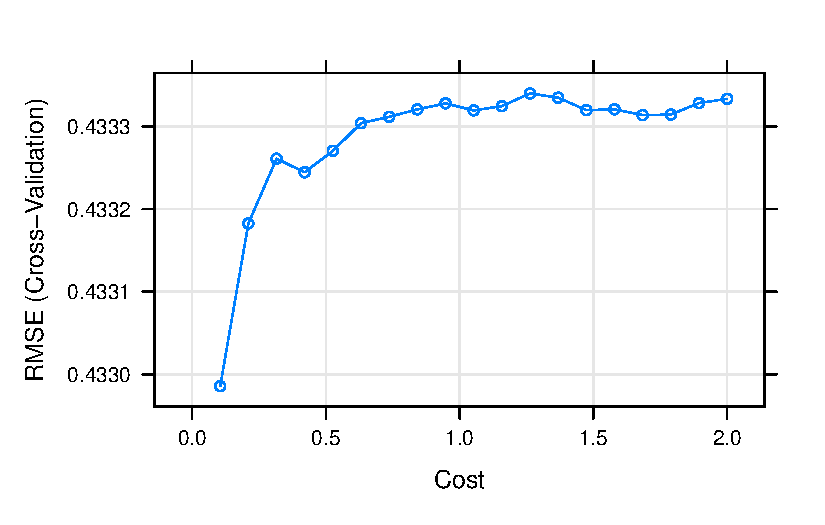
\includegraphics{AssignmentAdvancedTopicsInStatistics_files/figure-pdf/unnamed-chunk-22-1.pdf}

}

\end{figure}

\begin{Shaded}
\begin{Highlighting}[]
\CommentTok{\# Print the best tuning parameter C that maximises model accuracy}
\NormalTok{mdl}\SpecialCharTok{$}\NormalTok{bestTune}
\end{Highlighting}
\end{Shaded}

\begin{verbatim}
          C
2 0.1052632
\end{verbatim}

\#TODO talk about how there is a balance on how the number of miss
classified

\begin{Shaded}
\begin{Highlighting}[]
\DocumentationTok{\#\# the SVM not working part}

\CommentTok{\# \# Test model on testing data yTestPred \textless{}{-} predict(mdl,}
\CommentTok{\# newdata=X\_test) confusionMatrix(yTestPred, y\_test) \# predicted/true}
\end{Highlighting}
\end{Shaded}

\hypertarget{quick-debug-que-funciona-caralhoooooooooooooooo}{%
\subsection{quick debug que funciona
CARALHOOOOOOOOOOOOOOOO}\label{quick-debug-que-funciona-caralhoooooooooooooooo}}

\hypertarget{todo-this-is-using-radial-but-i-should-have-one-with-polynimial-as-well-to-show-that-polinomial-is-better}{%
\subsection{TODO this is using radial but I should have one with
polynimial as well to show that polinomial is
better}\label{todo-this-is-using-radial-but-i-should-have-one-with-polynimial-as-well-to-show-that-polinomial-is-better}}

\begin{Shaded}
\begin{Highlighting}[]
\DocumentationTok{\#\# https://github.com/MatheusSchaly/Online{-}Courses/blob/master/Machine\_Learning\_A{-}Z\_Hands{-}On\_Python\_\%26\_R\_In\_Data\_Science/2\_Classification/R/4\_Kernel\_SVM.R}
\DocumentationTok{\#\# to add visualization}

\NormalTok{mdl }\OtherTok{\textless{}{-}} \FunctionTok{train}\NormalTok{(}\AttributeTok{x=}\NormalTok{X\_train,}\AttributeTok{y=}\NormalTok{y\_train, }\AttributeTok{method=}\StringTok{\textquotesingle{}svmRadial\textquotesingle{}}\NormalTok{) }
\FunctionTok{print}\NormalTok{(mdl)}
\end{Highlighting}
\end{Shaded}

\begin{verbatim}
Support Vector Machines with Radial Basis Function Kernel 

800 samples
  2 predictor

No pre-processing
Resampling: Bootstrapped (25 reps) 
Summary of sample sizes: 800, 800, 800, 800, 800, 800, ... 
Resampling results across tuning parameters:

  C     RMSE       Rsquared   MAE      
  0.25  0.3165339  0.6025039  0.2003828
  0.50  0.3139614  0.6107481  0.1952854
  1.00  0.3113789  0.6183418  0.1920298

Tuning parameter 'sigma' was held constant at a value of 1.432896
RMSE was used to select the optimal model using the smallest value.
The final values used for the model were sigma = 1.432896 and C = 1.
\end{verbatim}

\begin{Shaded}
\begin{Highlighting}[]
\NormalTok{mdl }\OtherTok{=} \FunctionTok{svm}\NormalTok{(Group }\SpecialCharTok{\textasciitilde{}}\NormalTok{ .,}
                 \AttributeTok{data =}\NormalTok{ train,}
                 \AttributeTok{type =} \StringTok{\textquotesingle{}C{-}classification\textquotesingle{}}\NormalTok{,}
                 \AttributeTok{kernel =} \StringTok{\textquotesingle{}radial\textquotesingle{}}\NormalTok{)}

\CommentTok{\# Test model on testing data}
\NormalTok{yTestPred }\OtherTok{=} \FunctionTok{predict}\NormalTok{(mdl, }\AttributeTok{newdata=}\NormalTok{test)}
\CommentTok{\# yTestPred \textless{}{-} mdl \%\textgreater{}\% predict(xTest) }
\FunctionTok{confusionMatrix}\NormalTok{(}\FunctionTok{as.factor}\NormalTok{(yTestPred), }\FunctionTok{as.factor}\NormalTok{(y\_test)) }\CommentTok{\# predicted/true}
\end{Highlighting}
\end{Shaded}

\begin{verbatim}
Confusion Matrix and Statistics

          Reference
Prediction  0  1
         0 80 20
         1 15 85
                                         
               Accuracy : 0.825          
                 95% CI : (0.7651, 0.875)
    No Information Rate : 0.525          
    P-Value [Acc > NIR] : <2e-16         
                                         
                  Kappa : 0.65           
                                         
 Mcnemar's Test P-Value : 0.499          
                                         
            Sensitivity : 0.8421         
            Specificity : 0.8095         
         Pos Pred Value : 0.8000         
         Neg Pred Value : 0.8500         
             Prevalence : 0.4750         
         Detection Rate : 0.4000         
   Detection Prevalence : 0.5000         
      Balanced Accuracy : 0.8258         
                                         
       'Positive' Class : 0              
                                         
\end{verbatim}



\end{document}
